% \documentclass{report}
\documentclass[12pt]{report}
%\documentclass[a4paper,12pt]{report}

% IMPORT PACKAGE
\usepackage{lmodern}
\usepackage{hyperref}
\usepackage[T1]{fontenc}
\usepackage{geometry} 
\usepackage{graphicx}
\usepackage[french]{babel}
\usepackage{tikz}
\usetikzlibrary{calc}
\usepackage{fancyhdr}
\usepackage{titlesec}
\usepackage{listings}
\usetikzlibrary{shapes, arrows}

% PADDING
\geometry{
  a4paper,
  left=20mm,
  right=20mm,
  headheight=2cm,
  top=3cm,
  bottom=5cm,
  footskip=4cm
}

% Insérer une page blanche sans en-tête et sans pied de page
\newcommand\EmptyPage{
    \newpage
    \null
    \thispagestyle{empty}
    \addtocounter{page}{-1}
    \newpage}

\hypersetup{
    colorlinks=true,
    linkcolor=blue,
    filecolor=magenta,
    urlcolor=cyan,
}


% FRONT COVER
\renewcommand{\titlepage}{%
  \begin{tikzpicture}[remember picture,overlay]
    \node[inner sep=0pt] at (current page.center) {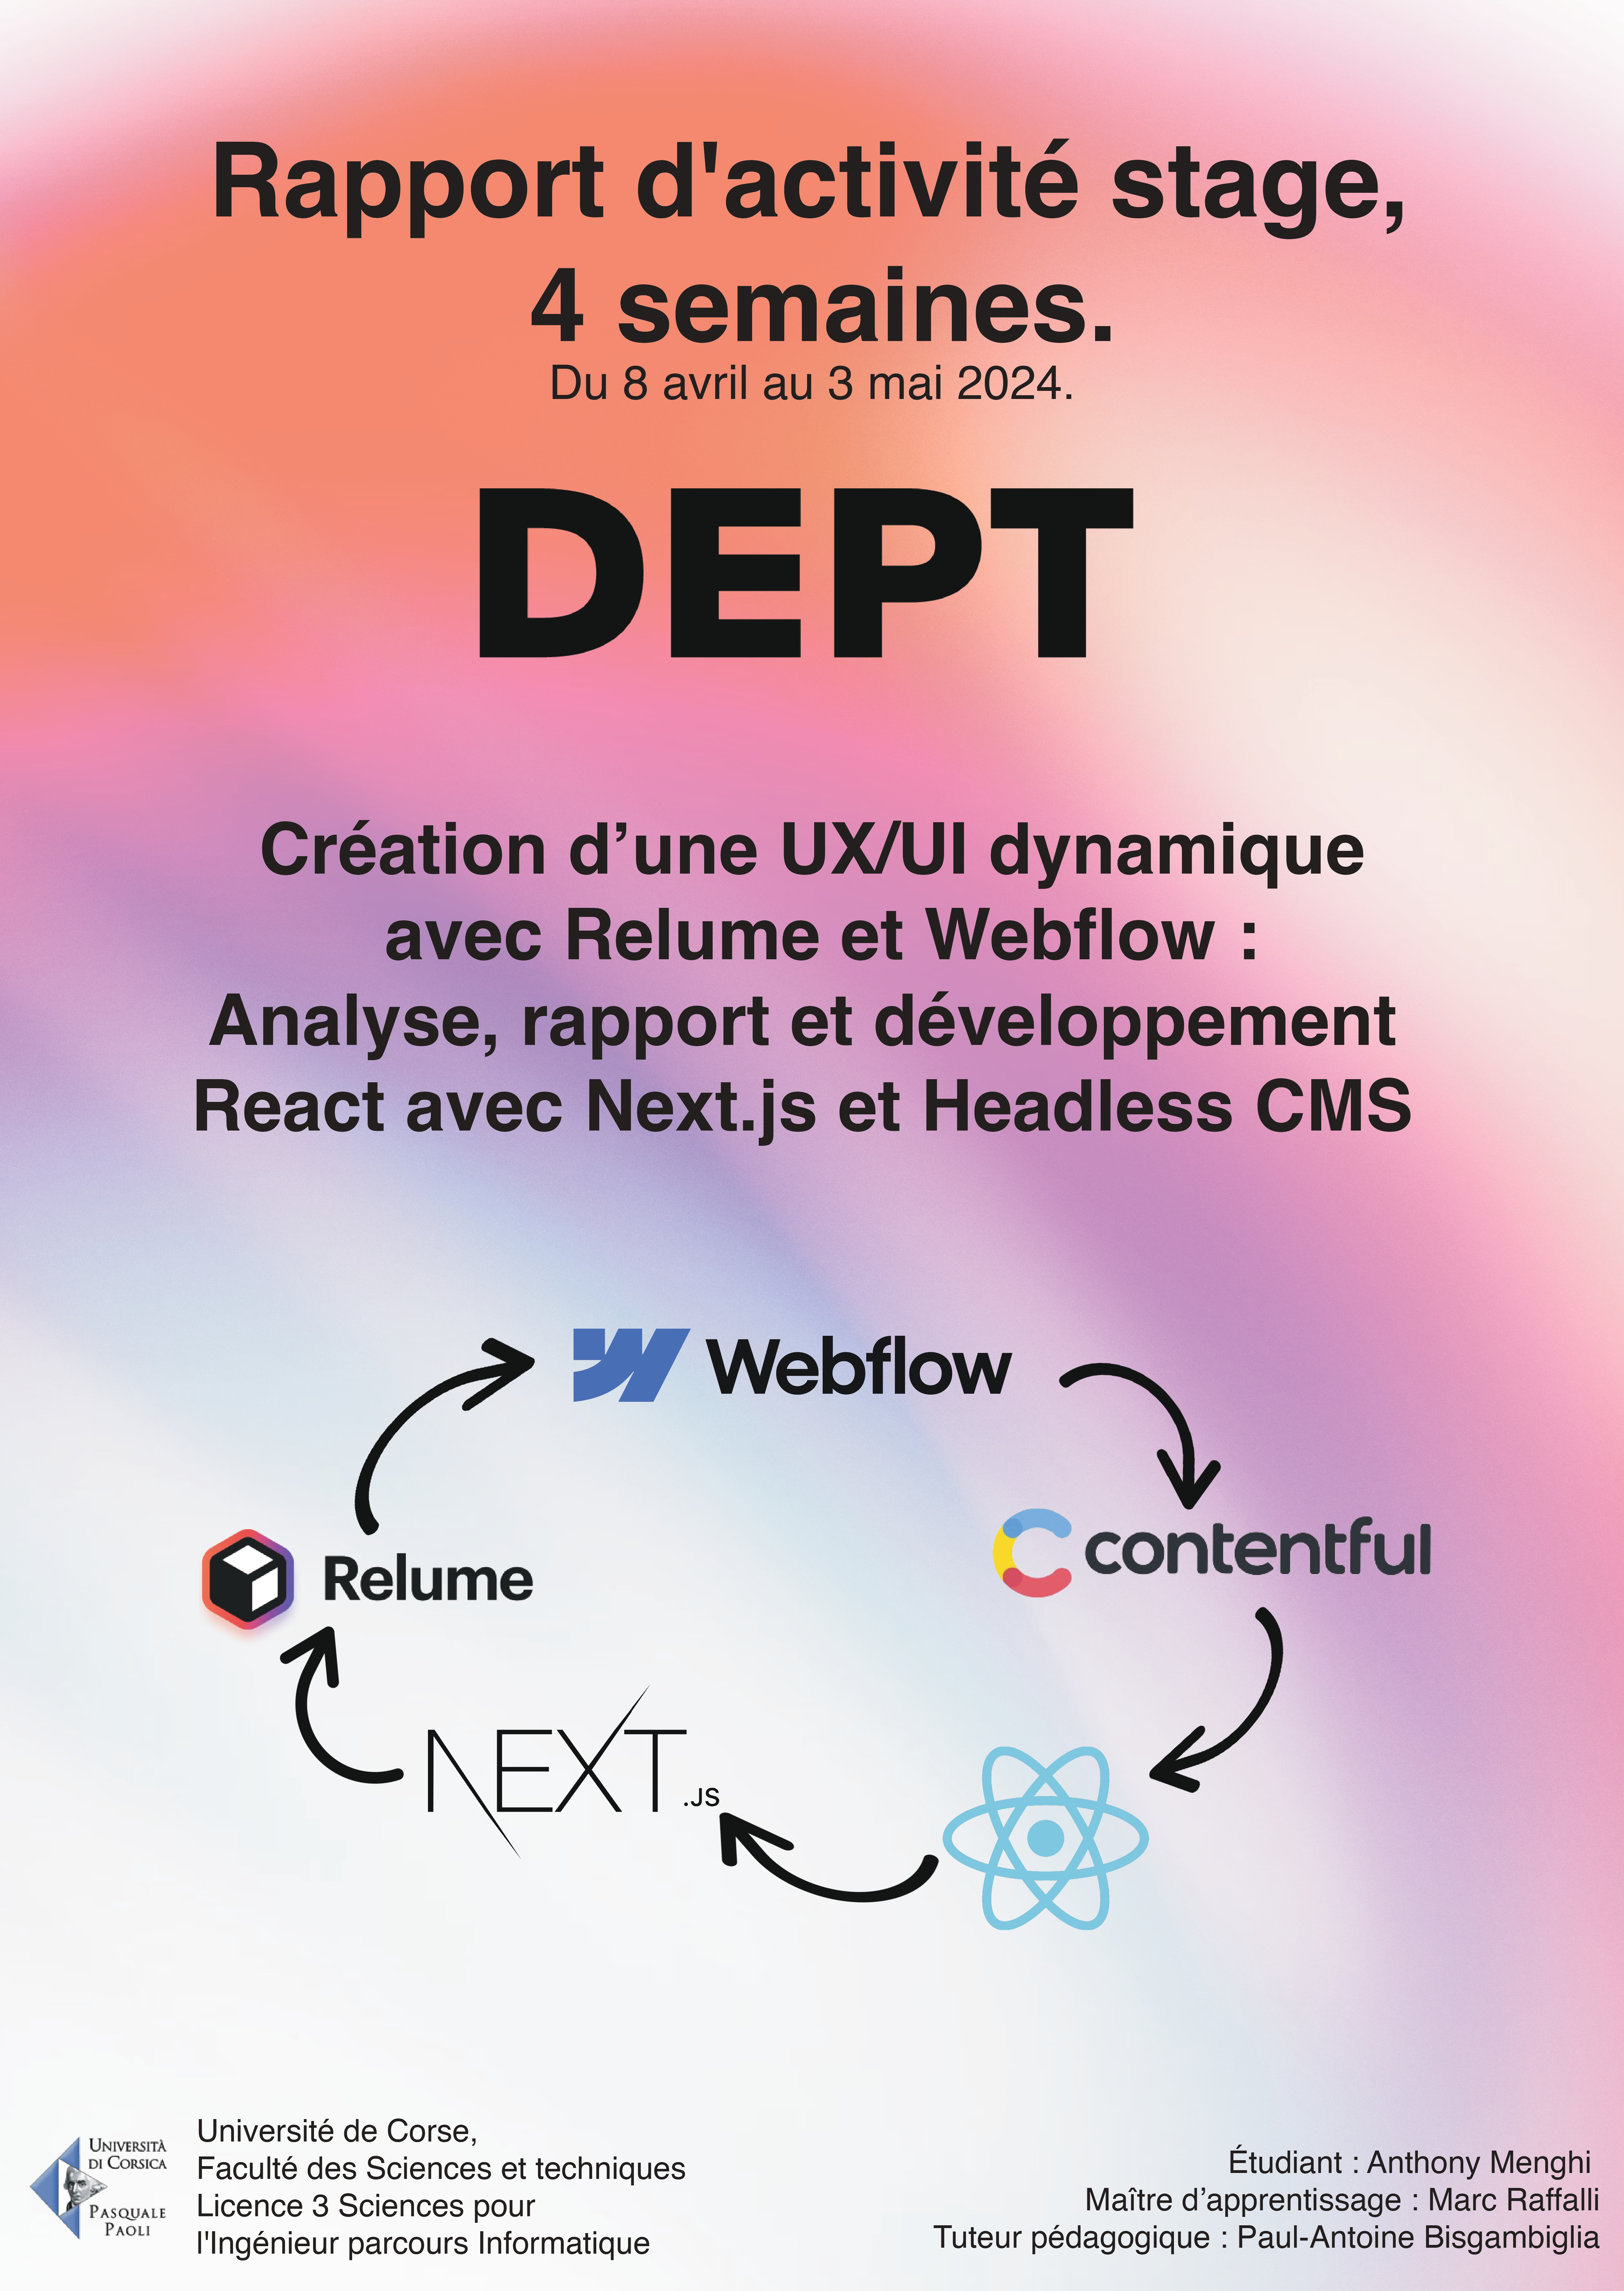
\includegraphics[width=\paperwidth,height=\paperheight]{Includes/Images/pageDeGarde2.jpg}};
  \end{tikzpicture}%
}

% HEAD & FOOTER
\pagestyle{fancy}

\fancyhead[L]{\includegraphics[width=2cm]{Includes/Images/Dept_Marketplaces_Logo.png}}
\fancyhead[C]{Rapport d'activité stage, 4 semaines.}
\fancyhead[R]{\includegraphics[width=1.5cm]{Includes/Images/universitedecorse.png}}

\fancyfoot[L]{Anthony Menghi}
\fancyfoot[C]{\thepage}
\fancyfoot[R]{\today}

\fancypagestyle{plain}{\pagestyle{fancy}}

% \fancypagestyle{plain}{% Redefine plain style
%     \fancyhf{} % Clear header and footer

%     \fancyhead[R]{\includegraphics[width=2cm]{Includes/Images/universitedecorse.png}}
  
%     % Includes/Images/universitedecorse.png
%     \fancyhead[C]{Rapport d'activité stage, 4 semaines.}

%     \fancyhead[L]{\includegraphics[width=2cm]{Includes/Images/Dept_Marketplaces_Logo.png}}
    

%     \fancyfoot[R]{18/05/2024} % Ajout du comptage de page
%     \fancyfoot[C]{\thepage}
%     \fancyfoot[L]{Anthony Menghi}
% }
% % Apply "plain" page style to all pages
% \pagestyle{plain}

% \title{Rapport de Stage - BUT MMI 2 \\ \Large Università di Corsica Pasquale Paoli}
% \author{Anthony Menghi}
% \date{June 2023}
\title{}
\author{}
\date{}

\begin{document}
\thispagestyle{empty} %enelver le page de style sur la page de couverture 
\maketitle 
\EmptyPage
% COVER PAGE
% UNIVERSITY
\vspace*{1cm}

\textbf{\Large Rapport d'activité de stage de 4 semaines}
\vspace*{0.8cm}

\textbf{Création d'une UX/UI dynamique avec Relume et Webflow : Anaylse, rapport et développement React avec Next.js et Headless CMS}
\vspace*{1cm}

\textbf{\underline{\Large Université :}}

\begin{figure}[h]
\includegraphics[width=0.15\textwidth]{Includes/Images/universitedecorse.png} 
\end{figure}

\begin{flushleft}
    \hspace{1cm} Università di Corsica Pasquale Paoli \\
    \hspace{1cm} Faculté des Sciences et techniques.\\
    \hspace{1cm} Campus Grimaldi, BP 52, 20250, Corte, France.\\
\end{flushleft}
\vspace{0.8cm}


% LABORATORY
\textbf{\underline{\Large Entreprise :}}

\begin{figure}[h] 
\includegraphics[width=0.2\textwidth]{Includes/Images/Dept_Marketplaces_Logo.png} 
\end{figure}

\begin{flushleft}
    \hspace{1cm} DEPT® \\
    \hspace{1cm} Full service digital agency - Pioneering tech/marketing \\
    \hspace{1cm} 24 Earlsfort Terrace,\\
    \hspace{1cm} D02 KC42, \\
    \hspace{1cm} Dublin , Ireland \\
\end{flushleft}
\vspace{0.8cm}


% STUDENT
\textbf{\underline{\Large Étudiant :}}
\begin{flushleft}
    \hspace{1cm} Anthony MENGHI, \\
    \hspace{1cm} Filière : Licence 3 Sciences pour l'Ingénieur \\
    \hspace{1cm} Parcours : Informatique, \\
    \hspace{1cm} Promotion : 2023. \\
\end{flushleft}
\vspace{0.8cm}
\textbf{\underline{\Large Maître d'apprentissage :}} 
\begin{flushleft}
    \hspace{1cm} M. Marc Raffali \\
    \hspace{1cm} Email : raffalli.marc.ed@gmail.com\\
\end{flushleft}
\vspace{0.8cm}

\textbf{\underline{\Large Tuteur pédagogique:}}  
\begin{flushleft}
    \hspace{1cm} M. Paul-Antoine Bisgambiglia \\
\end{flushleft}
\vspace{0.8cm}

\textbf{\underline{\Large Perdiode de stage :}}  
\begin{flushleft}
    \hspace{1cm} Du 8 avril au 3 mai 2024. \\
\end{flushleft}

\EmptyPage
\chapter*{Engagement de non plagiat}

Je, soussigné, Menghi Anthony, déclare être pleinement conscient que le plagiat de documents ou d’une partie d’un document publiés sur toutes formes de support, y compris l’internet, constitue une violation des droits d’auteur ainsi qu’une fraude caractérisée.  \\
En conséquence, je m’engage à citer toutes les sources que nous avons utilisées pour écrire ce rapport.
\EmptyPage

% NOTE READER
\chapter*{Note de lecture}


Cher lecteur, \\

Ce rapport contient des termes techniques couramment utilisés dans le domaine de l'informatique, tels que l'API, Headless CMS, etc. Des définitions de ces termes sont fournis via des notes de bas de page tout au long du texte, à partir de l'introduction. \\
Ces ressources vous aideront à mieux appréhender les concepts techniques présentés dans ce rapport. \\ 

Cordialement, \\ 

Anthony Menghi.
\EmptyPage
% ABSTRACTS
\chapter*{Synthèse}

Ce stage s'inscrit au sein de l'entreprise DEPT, au sein du département irlandais. DEPT est une entreprise pionnière en technologie et en marketing qui aide ses clients à garder une longueur d'avance. C'est une agence numérique à service complet, avec une équipe de plus de 4 000 spécialistes du numérique répartis sur plus de 30 sites sur cinq continents. Elle travaille à l'échelle mondiale avec des clients renommés tels qu'Adidas, Patagonia, Google Workspace et bien d'autres. DEPT combine narration créative et technologie pour créer des expériences numériques complètes, optimisant tout le parcours client. De plus, elle conçoit, construit et intègre des logiciels et du matériel pour les principales entreprises SaaS et traditionnelles.

Au cours de ce stage, ma mission a été de tester différents services, mettre en relation des outils, développer des solutions informatiques pour créer une UI et une UX totalement dynamiques. Afin de résoudre plusieurs problèmes comme la répétition du travail, le manque de synergie entre différents métiers tels que les designers graphiques, les content managers et les développeurs.

La solution développée pendant le stage permet de connecter la création de wireframes, le style graphique, le code et le contenu des pages en quelques clics pour permettre une meilleure expérience de travail et de relation entre les différents processus de création, afin de gagner en efficacité.

Ce stage m'a permis de découvrir le travail dans une entreprise internationale, l'ingénierie, la mise en place de projets, notamment en termes de gestion de projet, de processus d'automatisation et de différentes méthodes de travail. J'ai également eu l'opportunité de découvrir différents outils et services à la pointe de la technologie. J'ai également pu renforcer mes compétences en développement web en testant et en développant avec JavaScript, React et Next.js. Enfin, j'ai appris de nouvelles façons de coder avec l'apprentissage de nouveaux motifs d'architecture logicielle, de nouveaux outils et une nouvelle approche de l'utilisation de l'intelligence artificielle.

Grâce à ce stage, j'ai pu participer à un projet concret qui m'a permis de découvrir la mise en place et la réflexion de projets dans une entreprise internationale.
\\ \\
\textbf{Mots-clés :} Processus d'automatisation, Développement web, JavaScript, React, Next.js, Headless CMS, Service d'intelligence artificielle, Méthodes de travail, Motifs d'architecture logicielle, Gestion de projet.

\EmptyPage
% \include{Includes/Abstracts/abstract}
% \EmptyPage
% \include{Includes/Abstracts/riassuntu}
% \EmptyPage
% ACKNOWLEDGEMENTS
% \chapter*{Remmerciements}

Je tiens tout d'abord à exprimer ma profonde gratitude envers les personnes qui ont contribué à la réussite de mon stage et à mon enrichissement personnel. Je souhaite adresser mes sincères remerciements à :

\begin{itemize}

\item Mme Lucile Rossi, ma tutrice de projet au sein du projet GOLIAT. Je lui suis reconnaissant de m'avoir offert cette opportunité de stage et de m'avoir accompagné tout au long de cette expérience. Son expertise, son soutien et ses conseils précieux ont grandement contribué à la réalisation de mes objectifs.

\item M. Antoine Burglin, ingénieur de recherche, qui m'a aidé tout au long de mon stage. Sa disponibilité, ses compétences et sa bienveillance ont été essentielles dans mon apprentissage quotidien et dans la réussite de mes missions. Je le remercie chaleureusement pour sa patience et ses précieux conseils.

\item L'équipe pédagogique de la filière BUT MMI. Je souhaite exprimer ma gratitude envers les enseignants et les membres du personnel administratif qui ont contribué à ma formation et qui ont toujours été présents pour répondre à mes questions et me guider dans mon parcours.

\item L'équipe de l'administration du projet GOLIAT. Leur soutien logistique et administratif a grandement facilité le bon déroulement de mon stage. Leur disponibilité et leur professionnalisme ont été des atouts précieux dans la gestion du projet.

\item L'IUT de Corse et l'Université de Corse pour avoir mis à ma disposition les infrastructures nécessaires à la réalisation de mon stage. Leur soutien logistique et administratif a grandement facilité le bon déroulement de cette expérience professionnelle.
\end{itemize}

Enfin, je tiens à remercier tous ceux qui, de près ou de loin, ont contribué à la réussite de mon stage, notamment mes collègues de travail qui ont partagé leurs connaissances et leur expérience avec générosité. Leur implication et leur soutien ont été des facteurs déterminants dans l'enrichissement de mes compétences et dans la réussite de ce stage.

Je leur suis profondément reconnaissant et je garde un souvenir précieux de cette expérience.
% \EmptyPage
% TABLES OF COTENT
\tableofcontents
\EmptyPage
% INTRODUCTION
\chapter{Introduction}

Ce rapport de stage retrace mon expérience au sein de l'entreprise DEPT, dans son département irlandais. DEPT est une entreprise innovante dans les domaines de la technologie et du marketing, permettant à ses clients de toujours rester en avance. En tant qu'agence numérique proposant une gamme complète de services, DEPT réunit plus de 4 000 experts en numérique, répartis sur plus de 30 sites à travers cinq continents. Collaborant à l'échelle mondiale avec des clients prestigieux comme Adidas, Patagonia, Google Workspace, et bien d'autres, DEPT marie la narration créative à la technologie pour offrir des expériences numériques globales, optimisant ainsi chaque étape du parcours client. En outre, l'entreprise conçoit, développe et intègre des logiciels et du matériel pour les principales sociétés SaaS et traditionnelles.

Dans le cadre de mon stage, ma mission consistait à tester divers services, interconnecter des outils et développer des solutions informatiques visant à créer une interface utilisateur (UI) et une expérience utilisateur (UX) entièrement dynamiques. L'objectif était de résoudre plusieurs problématiques, notamment la répétition des tâches et le manque de synergie entre différents métiers comme les designers graphiques, les content managers et les développeurs.

Le présent rapport se concentre plus particulièrement sur ma contribution au développement d'une solution innovante permettant de relier différents outils pour intégrer la création de wireframes, le style graphique, le code et le contenu des pages en seulement quelques clics. Cela visait à améliorer l'expérience de travail et la collaboration entre les différents processus créatifs, afin d'accroître l'efficacité.
\\ \\
La première partie de ce rapport présente le contexte général du projet. J'y expose mes motivations personnelles qui m'ont conduit à m'engager dans ce stage, ainsi que les objectifs et les projets de l'entreprise DEPT. Je détaille également le cahier des charges, la gestion du temps pendant le stage et la gestion des projets au sein de l'entreprise.


La deuxième partie constitue le cœur de mon travail durant ce stage. J'y décris l'intégration des différents outils en suivant plusieurs étapes. Tout d'abord, je présente ces outils en détail, en soulignant leurs fonctionnalités et leur utilité. Ensuite, j'expose les réflexions sur les diverses possibilités d'interactions entre ces outils, en expliquant les choix technologiques et les stratégies adoptées.

La troisième partie se concentre sur la logique de développement avec un Headless CMS, développée en collaboration avec l'équipe du projet. J'y détaille le processus de réflexion, les décisions prises et les raisons derrière ces choix.


Enfin, je termine par une analyse critique de la solution développée, en présentant ses avantages et ses inconvénients. Cette évaluation permet de mettre en lumière les points forts du projet tout en identifiant les axes d'amélioration possibles pour l'avenir.
\\ \\
Je conclurai ce rapport en mettant en évidence les compétences que j'ai développées tout au long de mon stage, notamment en matière de développement web, de gestion de projet et de résolution de problèmes. Je soulignerai l'importance du travail d'équipe etl'exploration de nouvelles technologie. Ce rapport permettra ainsi de mieux appréhender les différentes étapes de mon travail, les solutions techniques que nous avons apportées

\EmptyPage
% CONTEXT
% CONTEXT
\chapter{Contexte et cahier des charges}


% PERSONAL PERSPECTIVES
\section{Perspectives personnelles}
Cette expérience professionnelle s'inscrit dans le cadre de mon stage de fin d'année en Licence 3 Sciences pour l'Ingénieur, parcours Informatique, à la Faculté des Sciences et Techniques de l'Université de Corse. J'ai été accueilli par l'entreprise DEPT, au sein de son département en Irlande.

J'ai choisi ce stage afin d'approfondir mes connaissances dans le domaine du web, de découvrir le monde de l'entreprise et de comprendre les méthodes de travail dans un contexte international. Cette opportunité de travailler dans une entreprise située hors de France m'a permis de découvrir de nouvelles pratiques professionnelles. Je suis très honoré de pouvoir apporter, à mon modeste niveau, une contribution à une entreprise de portée mondiale.


% PRESENTATION UNIV & PROJECT
\section{Présentation de DEPT et ses projets}
\subsection{Présentation}
DEPT a été créer en 2005 à Amsterdam au Pays-Bas c'est une entreprise innovante dans les domaines de la technologie et du marketing, aidant ses clients à rester à la pointe. En tant qu'agence numérique complète, DEPT réunit plus de 4 000 experts répartis sur plus de 30 sites à travers cinq continents. Travaillant avec des clients prestigieux tels qu'Adidas, Patagonia, Google Workspace, et bien d'autres, DEPT combine créativité et technologie pour offrir des expériences numériques globales, optimisant chaque étape du parcours client. De plus, l'entreprise conçoit, développe et intègre des solutions logicielles et matérielles pour les principales sociétés SaaS et traditionnelles.

\subsection{Projets de l'entreprise}
Du commerce électronique et des technologies émergentes aux expériences client et à l'architecture \footnote{Le cloud est un ensemble de serveurs distants utilisés pour stocker, gérer et traiter des données via Internet.}cloud, Dept imaginne et met en œuvre des solutions techniques d'avenir qui établissent de nouvelles normes pour les entreprises numériques.
\\ \\
DEPT a réalisé de nombreux projets en voici des exemples.


\subsubsection{Arizona State University}

DEPT collabore avec l'Arizona State University (ASU) pour rendre l'éducation plus accessible et équitable à travers le développement de plateformes éducatives adaptées aux besoins spécifiques des apprenants du monde entier. Depuis plus de six ans, DEPT et ASU ont créé diverses solutions EdTech, notamment:

\begin{itemize}
    \item \textbf{Baobab}: Application pour le réseautage et le mentorat des jeunes leaders africains.
    \item \textbf{me3®}: Outil interactif de planification de carrière basé sur un modèle \footnote{SaaS signifie "logiciel en tant que service". C'est un modèle où les logiciels sont hébergés sur le cloud et accessibles via Internet.}SaaS.
    \item \textbf{Young Thinkers}: Programme en ligne de préparation à l’université et à la carrière pour les jeunes émiratis et arabes.
    \item \textbf{Intelligent Tutor}: Tuteur intelligent pour l'apprentissage autonome en mathématiques.
\end{itemize}

En utilisant une approche centrée sur l'utilisateur, DEPT garantit que chaque solution est adaptée aux contraintes techniques et culturelles des apprenants, contribuant ainsi à démocratiser l'éducation et à atteindre plus d'un million d'utilisateurs à travers le monde.

\subsubsection{Fingerspelling}

HELLO MONDAY/DEPT® et l'American Society for Deaf Children ont créé \textbf{Fingerspelling.xyz}, une application web utilisant l'apprentissage automatique pour enseigner l'alphabet de la langue des signes américaine (ASL).

Fingerspelling.xyz utilise \textit{MediaPipe Hands} pour suivre les mouvements des mains via une webcam. Un modèle 3D montre comment positionner les mains pour chaque lettre, avec des retours en temps réel.

L'application a enregistré des millions de signes corrects et est utilisée par l'American Society for Deaf Children. Récompenses :
\begin{itemize}
    \item \textbf{Webby Awards 2023}: trois People's Voice Awards. 
    \item \textbf{Webby Awards 2022}: deux Webby Awards et trois People's Voice Awards.
    \item \textbf{Eurobest Awards}: Prix de l'innovation, Or en design.
    \item \textbf{Awwwards}: Site du jour.
    \item \textbf{FWA}: Site du jour et du mois.
    \item \textbf{Cannes Lions}: Or et Argent en design.
    \item \textbf{New York Design Awards 2021}: Argent.
    \item \textbf{Anthem Awards}: Or en Éducation.
\end{itemize}

Fingerspelling.xyz améliore la communication et l'inclusion pour la communauté des Sourds.

\subsection{Participation à l'entreprise}

Dept à de nombreux clients dans l'ecommerce et cherche à concevoir des solutions pour automatiser, éviter de la répétition de taches et améliorer la cohésion entre les différents professionnelles dans le processus de développement et de création
\\ \\
L’équipe qui s’occupe du développement de cet solution est composé de trois personnes : 
\begin{itemize}
    \item M. Derek Brady est le directeur créatif et associé chez DEPT, il s'occupe sur la vision à long terme de l'entreprise, il supervise et à dirige la création et le développement des aspects visuels et créatifs des projets.
    \item M. Marc Raffalli est développeur \footnote{Le front-end est la partie d'une application ou d'un site web avec laquelle les utilisateurs interagissent directement. Cela inclut l'interface utilisateur, le design et les fonctionnalités visibles.}front-end senior, il s'occupe de l'aspects techniques des projets, il s'est occupé de guider et de m'encadrer tout au long du stage
    \item Enfin, Moi-même, stagiaire ayant pour but de créer la solution pour optimier le processus de création avec l'UI et l'UX dynamique.
\end{itemize}

\section{Cahier des charges}
Le but de ce stage est de créer une solution pour automatiser pour la création d'UI et UX dynamique avec \footnote{JavaScript est un langage de programmation de haut niveau principalement utilisé pour créer des fonctionnalités interactives sur les sites web.}Javascript, \footnote{React est une bibliothèque JavaScript open-source utilisée pour construire des interfaces utilisateur interactives et réactives pour les applications web et mobiles.}React et \footnote{Next.js est un framework JavaScript basé sur React, utilisé pour créer des applications web rapides et évolutives.}Next.js pour les futurs clients de l'entreprise, en utilisant des technologies modernes et en respectant les standards de l'entreprise. 
\\ \\
Cette solution doit permettre de gagner du temps, d'éviter les erreurs et de faciliter la communication entre les différents professionnels.

Il m'a été demandé de tester plusieurs outils et services pour voir s'ils peuvent répondre aux problématiques.
Ensuite, il m'a été demandé d'étudier les différentes possiblité d'interactions entre les outils. 

Puis, de créer un prototype de la solution en utilisant Javascript \ref{doc:javascript} avec React \ref{doc:react} et Next.js \ref{doc:nextjs} connecté a un Headless CMS.

Enfin, de tester la solution, de identifié les forces et les faiblesses pour présenter la solution à l'équipe.

% Gestion du temps
\section{Gestion du temps}

Pendant mon stage, j'ai accordé une grande importance à une gestion efficace du temps, afin de maximiser ma productivité et de mener à bien les différentes tâches qui m'ont été confiées. Voici une vue d'ensemble de ma gestion du temps (figure \ref{fig:Diagramme circulaire - Gestion du temps}), basée sur les pourcentages suivants :

\begin{itemize}
\item \textbf{Programmation} : J'ai consacré environ 30\% de mon temps à la programmation. Cela inclut la création le développement en React et Next.js pour créer le prototype de la solution avec la connexion avec le Headless CMS et la mise en place du motif de conception.

\item \textbf{Test des outils} : Environ 25\% de mon temps a été dédié aux tests des outils. J'ai testé les outils Relume, Webflow et Devlink pour voir s'ils répondaient aux besoins du projet et pour identifier les avantages et les inconvénients de chacun.

\item \textbf{Recherche et apprentissage} : Environ 20\% de mon temps a été consacré à la recherche et à l'apprentissage de nouvelles technologies et des nouveaux outils. J'ai appris à utiliser des outils tels que Webflow, Relume et ContentFul pour le headless CMS, et j'ai approfondi mes connaissances en Next.js 14 qui a apporté des changements et nouvelles fonctionnalités.
\item \textbf{Collaboration} : J'ai consacré environ 15\% de mon temps à la collaboration avec l'équipe autour du projet. Cela comprenait des réunions, des discussions et des échanges d'idées pour garantir que le projet prenne la bonne direction, la prise en compte des éventuelles suggestions et la validation de l'avancée de projet.

\item \textbf{Analyse et proposition}: Environ 10\% de mon temps a été consacré à l'analyse des spécifications ; à la proposition de solutions adaptées aux besoins du projet et du cahier des charges. Cette phase m'a permis de comprendre en détail les exigences et d'identifier les meilleures approches pour les satisfaire.
\end{itemize}
\begin{figure}[ht] 
    \centering
    \includegraphics[width=0.7\textwidth]{Includes/Images/gestionTemps.png}
    \caption{Diagramme circulaire - Gestion du temps}
    \label{fig:Diagramme circulaire - Gestion du temps}
\end{figure} 
De ce fait, cette gestion du temps équilibrée m'a permis de mener à bien mes tâches et d'atteindre les objectifs fixés dans les délais impartis. Cette répartition réfléchie du temps m'a permis de rester organisé, de faire face aux défis et d'obtenir des résultats positifs tout au long de mon stage.

\subsection*{Communication et gestion de projets}

Pendant les quatres mois de mon stage, nous avons mis en place une solide gestion de projet, qui nous a permis de progresser de manière efficace et de répondre aux attentes fixées. Dès le début, j’ai reçu le cahier des charges détaillant les objectifs et les exigences du projet. Cela m’a donné une vision claire de ce qui était attendu et j’ai pu commencer à développer en conséquence.

Pour assurer un suivi régulier et des retours constructifs, j’ai adopté une approche itérative dans mon travail. À chaque petite étape ou module que je complétais, je les soumettais à M. Marc Raffalli, mon mentor et developpeur front-end senior. Il examinait attentivement mon travail et me fournissait des retours précieux. J’ai pris en compte ces commentaires et suggestions, ce qui m’a permis d’améliorer continuellement mes réalisations avant de passer à l’étape suivante.
\\ \\
Cette méthodologie agile a permis une flexibilité accrue, une adaptation en temps réel aux changements et une amélioration constante tout au long du processus de développement.

\EmptyPage
\chapter{Réalisations et création de la solution}
\section{Présentation des outils à conecter}

\subsection{Relume}

Relume \ref{doc:relume} est un outil innovant, conçu pour révolutionner la création de sites web grâce à l'intelligence artificielle. Il permet de générer rapidement des plans de site et des wireframes UX, tout en s'intégrant de manière fluide avec Figma\footnote{Figma est une plateforme de design collaborative basée sur le cloud, permettant aux équipes de créer, de prototyper et de collaborer sur des interfaces utilisateur et des designs interactifs.} et Webflow via un simple processus de copier-coller. 

De plus, Relume est particulièrement efficace pour les sites classiques, comme les sites e-commerce, qui utilisent souvent des composants récurrents tels que des carrousels, des barres de navigation, des pieds de page, etc.

C'est idéal pour les projets simples, Relume se distingue par sa capacité à augmenter la productivité tout en simplifiant la gestion des projets web. Toutefois, pour des projets plus complexes nécessitant des designs et des contenus plus personnalisés, l’intervention humaine reste indispensable. 

\subsection{Webflow}
Webflow \ref{doc:webflow} est une plateforme innovante de conception et de développement de sites web qui permet de créer des sites professionnels sans nécessiter de compétences en codage. Intégrant un éditeur visuel intuitif, Webflow permet de concevoir et de personnaliser des pages web à l'aide de fonctionnalités de glisser-déposer, tout en appliquant des styles CSS\footnote{Les styles CSS (Cascading Style Sheets) sont des règles utilisées pour définir l'apparence et la mise en page des éléments HTML sur une page web, comme les couleurs, les polices, les marges et les dimensions} en temps réel. Les capacités avancées d'interactions et d'animations permettent de créer des expériences utilisateur engageantes, sans écrire de code complexe. De plus, Webflow offre des possibilités de low code, permettant aux développeurs d'ajouter des fonctionnalités personnalisées à travers des snippets de code et des intégrations avec d'autres outils, enrichissant ainsi l'expérience et les capacités du site. Webflow représente ainsi une solution complète et accessible alliant design esthétique et performance technique.

\subsection{DevLink}
DevLink \ref{doc:devlink} constitue un outil de WebFlow qui facilite l'intégration des composants créés dans WebFlow à notre code (exclusivement React). Cette fonctionnalité permet d'exporter les composants créés dans WebFlow directement en code React via une simple ligne de commande. De surcroît, elle assure la synchronisation de nos composants dans notre code avec WebFlow. Ainsi, nous sommes en mesure d'importer les composants élaborés sur WebFlow dans notre code React, et de les mettre à jour automatiquement lorsque le designer effectue des modifications depuis WebFlow. 

\subsection{Contentful}
Contentful \ref{doc:contentful} est une plateforme de gestion de contenu (CMS headless) conçue pour répondre aux besoins des développeurs. Avec son architecture flexible basée sur le cloud et son API\footnote{Une API permet aux logiciels de communiquer entre eux en partageant des fonctionnalités ou des données.} robuste, Contentful offre une solution de gestion de contenu, les développeurs peuvent facilement intégrer Contentful à n'importe quelle technologie frontend grâce à ses API RESTful\footnote{Une API RESTful utilise HTTP pour effectuer des opérations sur des ressources} et GraphQL\footnote{GraphQL est un langage de requête, il permet aux clients de spécifier exactement les données dont ils ont besoin, ce qui évite le surchargement d'informations.}. Cela permet une séparation claire entre le backend\footnote{Le backend est la partie invisible d'une application qui gère les données et la logique de fonctionnement.} et le frontend, offrant ainsi une plus grande liberté de conception et une expérience de développement plus fluide. De plus, Contentful prend en charge la collaboration en équipe avec des fonctionnalités telles que les environnements de développement, les workflows\footnote{Les workflows sont des séquences d'étapes organisées pour accomplir une tâche ou un processus spécifique de manière efficace et cohérente.} de contenu et la gestion des droits d'accès, ce qui en fait un outil incontournable pour créer des expériences web dynamiques et évolutives.

\section{Réflexion sur les différentes possibilité d'interactions entre les outils}


\subsection{Possibilité n°1 - Basique}

Avec l'équipe nous avons réflechie sur les différentes possiblités d'interactions.

La première option, la plus basique, consiste à rassembler simplement les outils (voir figure \ref{fig: Schéma de la possibilité n°1 - Basique}). 
Le but est de créer le site sur Relume, qui génère toute l'expérience utilisateur (UX), les wireframes, les composants et le texte. Ensuite, nous transférons tout ce que nous avons construit sur Webflow pour créer l'interface utilisateur (UI), styliser le site, ajouter des animations, etc. Enfin, avec DevLink, nous exportons tous nos composants pour les intégrer dans notre code React. Cependant, tout le texte et le contenu sont codés en dur. Si nous souhaitons modifier le texte ou les images, nous devons resynchroniser DevLink et reconstruire le site avec Next.js.

\begin{figure}[h] 
  \centering
  \includegraphics[width=1\textwidth]{Includes/Images/connection1.png}
  \caption{Schéma de la possibilité n°1 - Basique}
  \label{fig: Schéma de la possibilité n°1 - Basique}
\end{figure} 

Cette méthode présente l'avantage de simplifier le processus initial de création et de design, mais elle impose des contraintes en termes de maintenance et de mises à jour de contenu. Pour chaque modification de texte ou d'image, il est nécessaire de passer par une étape de synchronisation et de reconstruction, ce qui peut être laborieux et chronophage.

\subsection{Possibilité n°2 - Avec un CMS}

Avec un CMS : L'objectif ici est de connecter Relume directement ou indirectement (via un webhook\footnote{Un webhook est un mécanisme permettant à une application de fournir des informations en temps réel à une autre application via des appels HTTP déclenchés par des événements.}) à un CMS, afin que Relume prenne en compte le texte du CMS et l'enregistre à chaque génération. Cela permet de rendre le texte modifiable dynamiquement dans le CMS et de ne pas le perdre à chaque régénération des wireframes.

\begin{figure}[h] 
  \centering
  \includegraphics[width=1\textwidth]{Includes/Images/connection2.png}
  \caption{Possibilité n°2 - Avec un CMS, option A}
  \label{fig: Possibilité n°2 - Avec un CMS, option A}
\end{figure} 

Option A (voir figure \ref{fig: Possibilité n°2 - Avec un CMS, option A}) : Connecter Relume directement à un CMS, puis de récupérer les données dans l'application React ou Webflow. Cette méthode permet de garder le contenu générer par Relume dans le CMS et de le récupérer dans l'application.

\begin{figure}[h] 
  \centering
  \includegraphics[width=0.6\textwidth]{Includes/Images/connection3.png}
  \caption{Possibilité n°2 - Avec un CMS, option B}
  \label{fig: Possibilité n°2 - Avec un CMS, option B}
\end{figure} 

Option B (voir figure \ref{fig: Possibilité n°2 - Avec un CMS, option B}) : Connecter Relume de manière indirecte à un CMS via un webhook, puis de récupérer les données dans l'application React ou Webflow.

Cette approche offre la flexibilité de modifier le contenu directement dans le CMS sans avoir à resynchroniser et reconstruire l'ensemble du site. Elle permet également de maintenir le contenu à jour plus facilement, bien que l'option B puisse impliquer des opérations supplémentaires pour gérer les webhooks.

\section{Développement de la solution}

Nous avons commencé à développer la solution en utilisant la première option pour tester les outils et comprendre leur fonctionnement. Nous avons réussi très facilement à connecter Relume à Webflow en suivant la documentation et les tutoriels vidéo réalisés par l'équipe de Relume. DevLink, bien qu'encore en version bêta, s'est avéré facile à utiliser. Il suffit de créer un fichier de configuration \texttt{.webflowrc.js}, d'ajouter les informations de connexion à Webflow, puis de lancer la commande \texttt{npx webflow devlink sync} pour exporter et synchroniser les composants de Webflow avec React. 
\\ \\
Ces outils sont très bien documentés et faciles à utiliser, ce qui nous a permis de les prendre rapidement en main. Cependant, comme mentionné précédemment, la première option présente des inconvénients en termes de maintenance et de mise à jour du contenu. C'est pourquoi nous avons décidé de nous concentrer sur la deuxième option, qui consiste à connecter Relume à un CMS pour gérer le contenu de manière dynamique.

Cette approche permet de modifier le contenu directement dans le CMS sans avoir à resynchroniser et reconstruire l'ensemble du site à chaque mise à jour. Elle améliore ainsi l'efficacité de la gestion du contenu et facilite les modifications ultérieures.
\\ \\ 
Lorsqu'on a commencé à explorer la possibilité de connecter Relume à un CMS, nous avons rencontré plusieurs difficultés. Relume est une plateforme très fermée, sans documentation officielle ni ressources en ligne pour connecter Relume à un CMS ou utiliser un WebHook. La documentation de Relume consiste principalement en vidéos YouTube \ref{doc:yb-relume}, qui ne sont pas adaptées à un développement durable ni aux besoins des développeurs. Une vidéo de la chaîne officielle de Relume, intitulée « Ajout de collections CMS aux composants | Relume Library » \ref{doc:relume-cms}, montre comment créer des composants avec des données provenant d'un CMS, mais cette opération est effectuée depuis Webflow et non depuis Relume.

Webflow propose son propre CMS, qui est stable et fonctionne très bien. Cependant, pour connecter un CMS externe comme Contentful, il faut « coder » cette opération en ajoutant du code JavaScript dans Webflow. Cette méthode complique l'utilisation de l'outil pour des utilisateurs non techniques, tels que les designers graphiques.

Nous avons donc décidé de repenser notre approche pour trouver une solution plus simple et plus efficace. 

\begin{figure}[h] 
  \centering
  \includegraphics[width=1\textwidth]{Includes/Images/connection4.png}
  \caption{Possibilité n°3 - Avec un CMS}
  \label{fig: Possibilité n°2 - Avec un CMS}
\end{figure} 

Nous avons envisagé une nouvelle (voir figure \ref{fig: Possibilité n°2 - Avec un CMS}) approche qui consiste à utiliser Relume pour générer les wireframes et les composants, que nous envoyons ensuite dans Webflow pour créer l'interface utilisateur (UI). Avec DevLink, nous transformons les composants Webflow en composants React et les intégrons dans notre code. Ensuite, nous connectons notre application React (Next.js) à un CMS (Contentful) pour gérer le contenu dynamique. Cette approche permet de bénéficier des avantages de chaque outil tout en simplifiant le processus de création et de gestion de contenu. Nous n'avons plus besoin de reconstruire le site à chaque modification de contenu, car nous récupérons directement le contenu du CMS en utilisant des requêtes API.

Cependant, nous devons synchroniser les composants de Webflow avec DevLink à chaque modification de ces composants et reconstruire le site pour voir les changements. Cette méthode combine la flexibilité du CMS pour la gestion dynamique du contenu avec la robustesse de Webflow et la puissance de React, tout en minimisant les efforts de maintenance.

\section{Logique de développement avec Headless CMS}
\begin{figure}[h] 
  \centering
  \includegraphics[width=0.8\textwidth]{Includes/Images/architecture.png}
  \caption{Architecture de la logique de développement avec Headless CMS}
  \label{fig: Architecture de la logique de développement avec Headless CMS}
\end{figure}

Pour créer la solution la plus flexible et la plus efficace possible, nous avons décidé d'utiliser un CMS headless pour gérer le contenu dynamique de notre application. Avec M. Marc Raffalli, développeur senior front-end et maître de stage, nous avons organisé plusieurs réunion pour discuter de la meilleure façon d'architecture front-end pour une connexion avec un CMS ; il m'a appris de noubreuses nouvelles façons d'apprenhender le développement front-end. La logique sous-jacente sortie de nos discussions est la suivante (voir figure \ref{fig: Architecture de la logique de développement avec Headless CMS}) :
Nous avons trois niveaux de composants.
\begin{itemize}
  \item \textbf{ContainerCMSPage}: Le but de ce component est d'implementer la logique de récupération des données d'un content type contenant les composants des pages. Le but ici est de créer la page en récupérant les composants de la page et de les afficher en donnant les props\footnote{"Props" est un raccourci pour "propriétés" en React. Ce sont des données passées d'un composant parent à un composant enfant, permettant la communication entre eux.} nécessaires à chaque composant.
  \item \textbf{ContainerCMSComponent}: Le but de ce composant est d'associé les données récupérer du CMS au composant Webflow.
  \item \textbf{Component}: Composant Webflow exporté avec DevLink.
\end{itemize}
\vspace{0.8cm}
Plus précisément, après avoir créer les wireframes et les composants sur Relume, styliser, animer sur Webflow et exporter les composants avec DevLink vers notre application. Nous créer des Content Type (un modèle de donnée comme un table en base de donneés) \ref{doc:contentful} pur chaque composant, nous créeons un Content Type qui sera une liste de composants pour chaque page. Ensuite, nous récupérons les données de chaque composant de la page et les affichons dans notre application en utilisant les composants Webflow exportés.

\section{Les avantages de cette solution et les inconvénients}

Une fois le prototype de la solution développé, nous avons pu constater les avantages et les inconvénients de cette approche du point de vue techniques et fonctionnels, nous parlerons pas des avantages et des inconvénients financiers, de dépendance, de sécurité, etc.

\subsection{Avantages}
\begin{itemize}
  \item Permet de synchroniser et d'améliorer la collaboration entre les différents métiers (designers, développeurs, content managers).
  \item Le développeur front-end n'a plus besoin de s'occuper de l'implémentation du composant mais peut se concentrer sur la partie logique, l'architecture, les tests, etc.
  \item La génération du code exporté par DevLink est lisible
\end{itemize}

\subsection{Inconvénients}
\begin{itemize}
  \item Certains composants Webflow ne sont pas compatible comme la collection list, les éléments ecommerce, les animations Lottie et les lightbox.
  \item Impossibilité de modifier les composants depuis React et avoir les changements sur Webflow, la synchronisation ne fonctionne que dans un sens.
  \item L'atomic design n'est pas gérée correctement, le code généré doit être modifié mais est écrasé lors de la prochaine synchronisation.
  \item Une partie du code généré est « inutile » et peut être difficile à lire si le composant est complexe notamment avec les animations.
  \item Erreurs de synchronisation sans explication et sans gestion des erreurs.
  \item Nous avons pas trouvé de solution pour créer des props avec une structure de données personnalisée (liste, tableau, json, etc.)
\end{itemize}



% DEVELOPMENT CONTEXT
% \include{Includes/contexteDeveloppement}
\EmptyPage

% creationInterface
% \include{Includes/creationInterface}
\EmptyPage
% CONCLUSIONS
% \chapter{Conclusion}
En conclusion, ce stage au sein du projet GOLIAT a été une expérience enrichissante et stimulante. J'ai réussi à réaliser toutes les fonctionnalités prioritaires définies dans le cahier des charges, démontrant ma capacité d'adaptation et d'intégration au sein du projet. J'ai conçu et développé toutes les pages de l'interface en respectant la charte graphique établie, en proposant un design moderne et soigné, avec une attention particulière portée à l'expérience utilisateur et à la compatibilité responsive sur différentes plateformes. Les composants essentiels tels que la barre de navigation et le tableau triable et responsive ont été implémentés avec succès.

La mise en place de toutes les fonctionnalités de l'API a été un élément clé de ma contribution au projet. J'ai assuré la connexion à l'API, la lecture des caméras, l'ajout des caméras, la gestion des opérations, y compris la suppression filtrée par leur statut, ainsi que le traitement des photos des opérations avec le téléversement et l'obtention des points chauds, qui sont ensuite visualisés sur une carte interactive. Toutes ces fonctionnalités sont opérationnelles et parfaitement intégrées à l'API existante, grâce à l'utilisation de Docker pour connecter et exécuter l'ensemble du projet avec une seule ligne de commande.

Ce stage m'a permis d'acquérir de nouvelles compétences et de renforcer mes connaissances dans divers domaines. J'ai pu approfondir mes compétences en développement web, en utilisant des technologies telles que Next.js, React et TypeScript, ainsi qu'en gestion de bases de données avec PostgreSQL. J'ai également développé mes compétences en matière de gestion de projet, de résolution de problèmes et d'adaptation.
Cette expérience m'a apporté une compréhension approfondie du travail dans la recherche et l'ingénierie, ainsi que des méthodes de travail efficaces.

Je suis fier d'avoir contribué de manière significative au projet GOLIAT en créant une interface web fonctionnelle qui répond aux exigences du cahier des charges. Mon travail a été apprécié par l'équipe et ils m'ont proposé un contrat à durée déterminée de deux mois pour poursuivre et améliorer l'interface web. Cette opportunité de prolonger mon engagement témoigne de la confiance qu'ils ont en mes compétences et de l'importance accordée à mon apport au projet.

En ce qui concerne mes perspectives d'avenir, je nourris l'ambition de devenir développeur full stack spécialisé dans les médias interactifs. Je souhaite continuer mes études et me perfectionner dans les domaines du développement web, de la conception d'interfaces et des technologies émergentes. Ce stage a confirmé mon idée et ma vocation dans ce domaine passionnant. Je suis motivé à poursuivre mon parcours, à acquérir de nouvelles compétences et à contribuer à des projets innovants qui allient technologie et créativité.

En somme, ce stage m'a permis de grandir professionnellement et personnellement. J'ai pu mettre en pratique mes connaissances, relever des défis techniques et contribuer à un projet concret visant à améliorer la lutte contre les feux de forêts. Je suis reconnaissant d'avoir participé à cette expérience et je suis impatient de continuer à contribuer au développement de l'interface web dans le cadre du contrat qui m'a été proposé.
\EmptyPage
% TABLES OF FIGURES
\listoffigures

\EmptyPage
% \include{Includes/annexe}

\end{document}




% Mise en relation des différents outils
% Découverte & tests
% Relume
% Webflow
% DevLink
% Reflexion sur les difféntes possibilité d'interactions entre les outils
% Logique de développement avec Headless CMS
% Les pour et les contres
% Conclusion
% Webographie
% Tables des figures
% Annexe